%==============================================================================
%== template for LATEX poster =================================================
%==============================================================================
%
%--A0 beamer slide-------------------------------------------------------------
\documentclass[final]{beamer}
\usepackage{etex} % too many packages in beamerposter
\usepackage[orientation=portrait,size=a0,
            scale=1.25         % font scale factor
           ]{beamerposter}
          
\usepackage{booktabs}
\geometry{
  hmargin=2.5cm, % little modification of margins
}

%
\usepackage[utf8]{inputenc}
\graphicspath{{figures/}} % Location of the graphics files
\newcommand{\abnet}{{\sc ABnet}}
\newcommand{\norm}[1]{\lVert#1\rVert}
\newcommand{\tup}[1]{\langle#1\rangle}

\linespread{1.05} %%% TODO CHANGE (was 1.15)
%
%==The poster style============================================================
\usetheme{sharelatex}

%==Title, date and authors of the poster=======================================
\title
[Interspeech (2015, Dresden, Germany)] % Conference
{ % Poster title
Hybrid Spoken Term Discovery-ABnet System\\
Finding words to learn segments
}

\author{ % Authors
Roland Thiolli\`ere\inst{*}, Ewan Dunbar\inst{*}, Gabriel Synnaeve\inst{*\dagger}, Maarten Versteegh\inst{*}, Emmanuel Dupoux\inst{*}
}
\institute
[ENS] % General University
{
\inst{*} LSCP, \'{E}cole Normale Sup\'{e}rieure / EHESS / CNRS, Paris, France\\%[0.3ex]
\inst{\dagger} now at Facebook AI Research\\[0.5ex]
\inst{} \begin{small}\texttt{rolthiolliere@gmail.com, emd@umd.edu, gabrielsynnaeve@gmail.com, maartenversteegh@gmail.com, emmanuel.dupoux@gmail.com}\end{small}
}
%\date{\today}


\begin{document}
\begin{frame}[t]
%==============================================================================
\begin{multicols}{3} % try 2
%==============================================================================
%==The poster content==========================================================
%==============================================================================

\section{Introduction}

\begin{itemize}
\item This system is the combination of two architectures: a spoken term discovery\cite{jansenvandurme2011} (STD) and a siamese neural network\cite{synnaevedupoux2014} (\abnet{}).
\item The STD system finds matching patterns in the acoustic signal.
\item The \abnet{} is trained to minimize the distance between those matching patterns, and maximize the distance between non matching patterns.
\end{itemize}


%-----------------------------------------
%	Motivation
%-----------------------------------------

\section{Motivation}

\begin{itemize}
\item The high level idea: two randomly selected words will be more distant in acoustic space than two randomly selected phonemes. It is easier to discriminate words than phonemes.
\item Our approach: extract word level information to learn phonemes.
\end{itemize}

%-----------------------------------------
%       SYSTEM
%-----------------------------------------

\section{System}

\vspace{0.5cm}
\begin{figure}[ht!]
  \begin{center}
    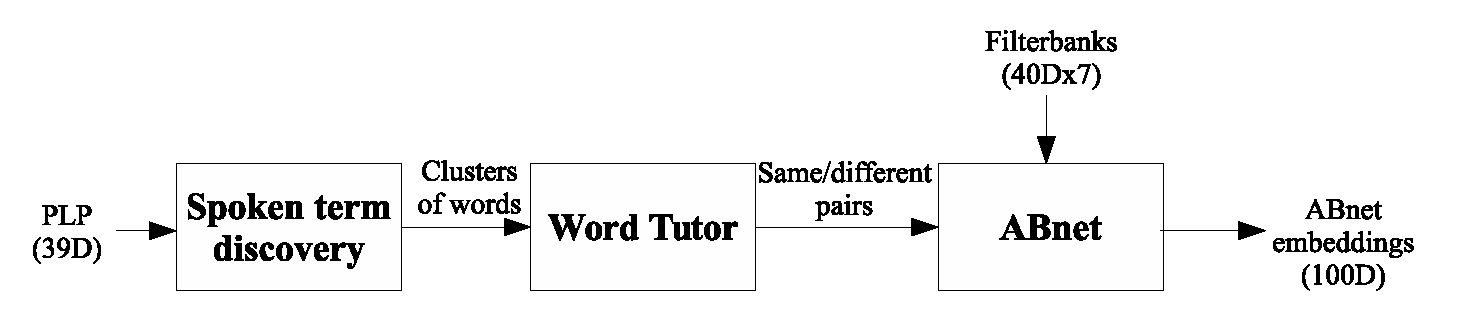
\includegraphics[width=\columnwidth]{system}
    \caption{\label{fig:system}Overview of the components of our system.}
  \end{center}
\end{figure}

A word tutor was designed to link the STD system and the \abnet{}. The 3 parts are described below.

%-----------------------------------------
%       SPOKEN TERM DISCOVERY
%-----------------------------------------

\subsection{Spoken term discovery}

\begin{itemize}
\item System used as baseline for track 2 \cite{versteeghetal2015}.
\item Finding patterns in an approximation of the similarity matrix.
\item Computes an approximation of the similarity matrix (cosine similarity).
\item Searches for diagonal patterns in that matrix.
\item Those matching patterns are then filtered and clustered.
\end{itemize}

See \cite{jansenvandurme2011} for more.

\begin{figure}[ht!]
  \begin{center}
    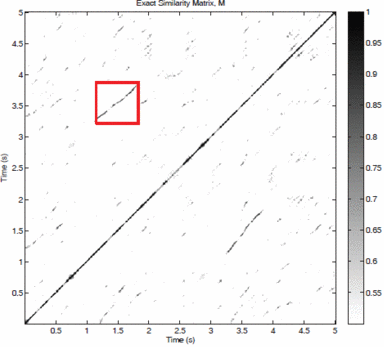
\includegraphics[width=0.4\columnwidth]{similarity_matrix}
    \caption{\label{fig:system}Similarity matrix of the signal. Source: \cite{jansenvandurme2011}}
  \end{center}
\end{figure}

\subsection{Word tutor}

\begin{itemize}
\item The word tutor selects the words that it will feed to the \abnet{}, making the link between the STD system and the \abnet{}.
\item Pairs of ``different'' words are randomly selected amongst the discovered patterns. All pairs of words (same and different) are DTW aligned.

\item We extract 40 dimensionnal log-energy Mel-scale filterbanks (10ms step and 25ms window size). 7 adjacent (following the ``aligned'' path for pairs of ``same'' words, no alignment for ``different'' words) frames are stacked as input for the \abnet{}.
\end{itemize}

\vfill
\columnbreak

\subsection{ABnet}

\begin{itemize}
\item The \abnet{} is a siamese neural network architecture: the weights in the second branch are the duplicate of the weights in the first branch.
\item Input: a pair of examples (A, B) and a label Y=(same|different), here 7 stacked frames of 40 dimensionnal filterbanks.
\item loss function = similarity if same, distance if different.

\vspace{1cm}
\begin{figure}[ht!]
  \begin{center}
    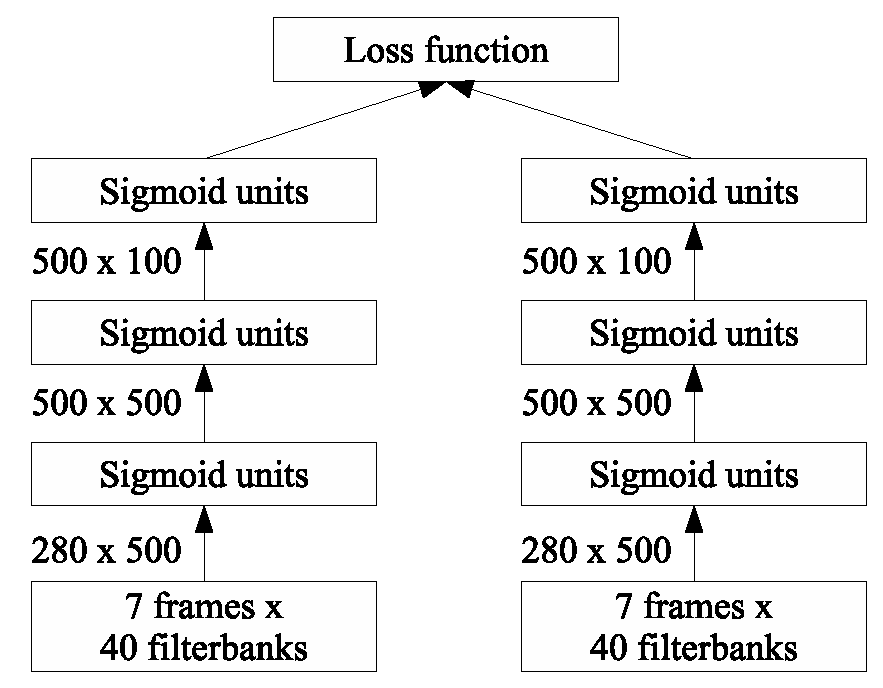
\includegraphics[width=0.85\columnwidth]{abnet}
    \caption{\label{fig:system}Overview of the components of our system.}
  \end{center}
\end{figure}

\item Loss function used:

\[
\mathcal{L}(A, B) =
\begin{cases}
(1-\cos(Y_A, Y_B)) / 2 & \text{if same} \\
\cos^2(Y_A, Y_B)       & \text{if different}
\end{cases}
\]

\noindent        
where $$\cos(x, y) = \frac{\tup{x, y}}{\norm{x}\norm{y}}$$

\item It learns a space where inputs with the same label are close together, and inputs with different labels are far appart. 
\end{itemize}

%-----------------------------------------
%	Extensions
%-----------------------------------------

\section{Extension: M-delta filtering}

\begin{figure}[ht!]
  \begin{center}
    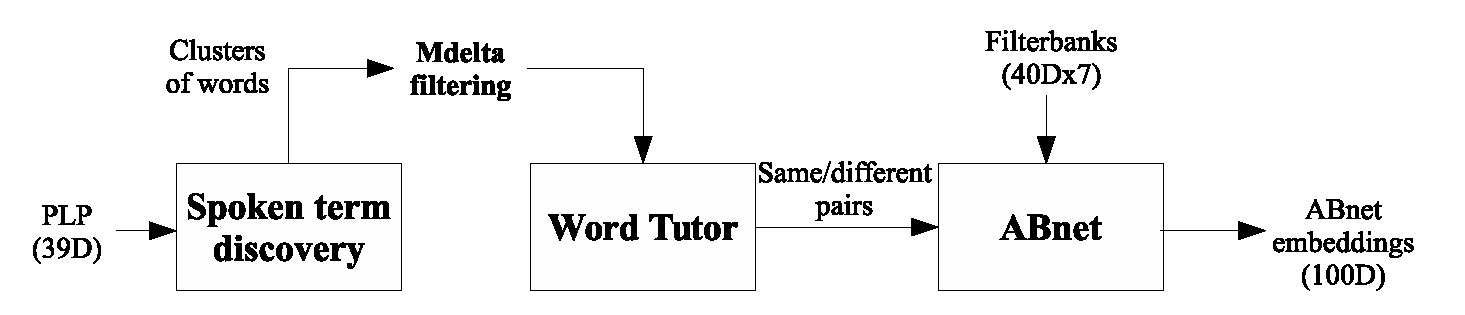
\includegraphics[width=\columnwidth]{system_mdelta}
    \caption{\label{fig:system}Overview of the components of our system.}
  \end{center}
\end{figure}

\subsection{Description}
\begin{itemize}
\item Two close frames (more likely to belong to the same phoneme) should differ less than two distant frames.
\item the M-delta measure\cite{ogawaetal2015} quantify how this property is verified.
$$M_\Delta = \mu{}_{\mathrm{across}} - \mu{}_{\mathrm{within}}$$
\item $\mu{}_{\mathrm{across}}$ (resp. $\mu{}_{\mathrm{within}}$) is an estimation of the average M-measure over frames belonging to different (resp. same) phonemes.
\item The M-measure is the average over all frames of the symmetric KL-divergence between 2 frames (here we used the cosine distance instead the divergence).
\end{itemize}

\subsection{Experiment}
\begin{itemize}
\item M-delta measure estimated locally for each frames, with a context of 500ms.
\item For each fragment found by the STD system, the average M-delta is calculated. The lower quartile is filtered out.
\end{itemize}
The results of the filtering are described in the next table. The NED is the normalized levenstein distance (calculated on the phone transcription). The coverage is a measure of the percentage of the corpus inventory discovered.

\begin{table}[h]
\caption{\label{tab:std-stats} Output of the spoken term discovery system. These fragments serve as input to the \abnet{}.}
\small
% \begin{tabular}{lccccccccccccccccc}
\begin{tabular}{lccccc}
\hline
         & Words & Pairs & Classes & NED   & Coverage \\
\hline
English & 6512 & 4305 & 3149 & 0.219 & 0.163 \\
English with Mdelta & 4334 & 2630 & 2092 & 0.229 & 0.106 \\
\hline
Xitsonga & 3582 & 1818 & 1782 & 0.120 & 0.162 \\
Xitsonga with Mdelta & 2286 & 1158 & 1138 &  \textbf{0.105} & 0.106 \\
\hline
\end{tabular}
\end{table}

\begin{itemize}
\item The filtering did improve the NED, but only for the Xitsonga dataset.
\end{itemize}

% \subsection{Speaker embedding}

% Adding speaker information.

% \begin{figure}[ht!]
%   \begin{center}
%     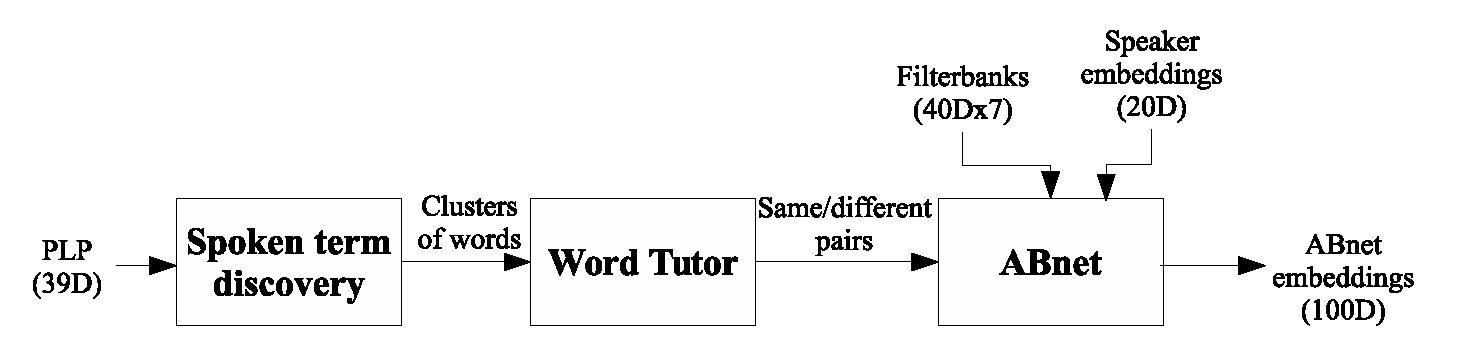
\includegraphics[width=\columnwidth]{system_spk}
%     \caption{\label{fig:system}Overview of the components of our system.}
%   \end{center}
% \end{figure}


%----------------------------------------------------------------------------------------
%	RESULTS 
%----------------------------------------------------------------------------------------

\section{Results}

\begin{itemize}
\item The speech representation is evaluated with the ABX paradigm (see \cite{versteeghetal2015}).
\item Two task: discriminate phones within speakers, and discriminate phones across speakers.

%
\vspace{1cm}
\begin{table}[htb]
\caption{ Within and across speaker Minimal Pair ABX error rates.}
\label{tab:track1}
\vspace{1cm}
\centerline{
\begin{tabular}{lcccc}
\hline
  & \multicolumn{2}{c}{\underline{English}}  & \multicolumn{2}{c}{\underline{Xitsonga}}    \\
  & Within  & Across   & Within  & Across   \\
\hline
  Baseline (MFCC)          & \emph{15.6}      & \emph{28.1}      & \emph{19.1}      & \emph{33.8}      \\
  Topline (HMM-GMM)           & \emph{12.1}      & \emph{16.0}      & \emph{3.5}       & \emph{4.5}      \\
\hline
STD $\rightarrow$ \abnet{} & \textbf{12.0}      & \textbf{17.9}      & \textbf{11.7}      & \textbf{16.6}      \\
STD / MDelta $\rightarrow$ \abnet{} & 12.4      & 18.1      & 12.6      & 18.6      \\
% STD + SpkID $\rightarrow$ \abnet{} & 12.2      & 18.0      & 16.5      & 21.3      \\
\hline
\end{tabular}
}
\end{table}
%
\item The overall system raised a substancial improvement over baseline.
\item Adding M-delta filtering did not improve the results.
\end{itemize}


%----------------------------------------------------------------------------------------
%	CONCLUSIONS
%----------------------------------------------------------------------------------------

% \color{SaddleBrown} % SaddleBrown color for the conclusions to make them stand out

\section{Conclusions}

\begin{itemize}
\item The results validate the approach. Despite the low number of examples, a good speech representation can be learnt.\\
\item However, all our attempts to further improve the results by adding additional information failed.
\end{itemize}

% \color{DarkSlateGray} % Set the color back to DarkSlateGray for the rest of the content

%----------------------------------------------------------------------------------------
%	FORTHCOMING RESEARCH
%----------------------------------------------------------------------------------------

\section{Forthcoming Research}

\begin{itemize}
\item Loop over the system (STD on learnt features).
\item Succesfully apply MDelta to STD output to improve track 2.
\end{itemize}

%----------------------------------------------------------------------------------------
%	REFERENCES
%----------------------------------------------------------------------------------------

\section{References}

\nocite{*} % Print all references regardless of whether they were cited in the poster or not
\bibliographystyle{IEEEtran} % Plain referencing style
\bibliography{bib} % Use the example bibliography file sample.bib

%----------------------------------------------------------------------------------------
%	ACKNOWLEDGEMENTS
%----------------------------------------------------------------------------------------

\section{Acknowledgements}

This work really was a team effort, all authors contributed equally.\\
We would like to thank Aren Jansen for letting us use his spoken term discovery system pre-release, and for his technical support.
%----------------------------------------------------------------------------------------

%--End of references-----------------------------------------------------------

\end{multicols}

%==============================================================================
\end{frame}
\end{document}

